%%%%%%%%%%%%%%%%%%%%%%%%%%%%%%%%%%%%%%%%%
% Journal Article
% LaTeX Template
% Version 1.3 (9/9/13)
%
% This template has been downloaded from:
% http://www.LaTeXTemplates.com
%
% Original author:
% Frits Wenneker (http://www.howtotex.com)
%
% License:
% CC BY-NC-SA 3.0 (http://creativecommons.org/licenses/by-nc-sa/3.0/)
%
%%%%%%%%%%%%%%%%%%%%%%%%%%%%%%%%%%%%%%%%%

%----------------------------------------------------------------------------------------
%	PACKAGES AND OTHER DOCUMENT CONFIGURATIONS
%----------------------------------------------------------------------------------------

\documentclass[fleqn]{IOS-Book-Article}
\usepackage{amsmath}
\usepackage{booktabs,array}
\newcolumntype{A}{@{}llccc >{$} r <{$} @{} >{${}} l <{$}@{}}
\usepackage{fancyhdr}
\usepackage{tikz}

\usepackage{relsize}
\usepackage{lipsum} % Package to generate dummy text throughout this template
\usepackage{graphicx}
\usepackage[sc]{mathpazo} % Use the Palatino font
\usepackage[T1]{fontenc} % Use 8-bit encoding that has 256 glyphs
\linespread{1.05} % Line spacing - Palatino needs more space between lines
\usepackage{microtype} % Slightly tweak font spacing for aesthetics

%\usepackage[hmarginratio=1:1,top=32mm,columnsep=20pt]{geometry} % Document margins
\usepackage{multicol} % Used for the two-column layout of the document
\usepackage[hang, small,labelfont=bf,up,textfont=it,up]{caption} % Custom captions under/above floats in tables or figures
\usepackage{booktabs} % Horizontal rules in tables
\usepackage{float} % Required for tables and figures in the multi-column environment - they need to be placed in specific locations with the [H] (e.g. \begin{table}[H])
\usepackage{hyperref} % For hyperlinks in the PDF

\usepackage{lettrine} % The lettrine is the first enlarged letter at the beginning of the text
\usepackage{paralist} % Used for the compactitem environment which makes bullet points with less space between them

%\usepackage{abstract} % Allows abstract customization
%\renewcommand{\abstractnamefont}{\normalfont\bfseries} % Set the "Abstract" text to bold
%\renewcommand{\abstracttextfont}{\normalfont\small\itshape} % Set the abstract itself to small italic text

\usepackage{pdfpages}
\usepackage{amssymb}
%[doi=false,issn=false,url=false,language=false, keywords=false]
\usepackage{natbib}
%\usepackage{titlesec} % Allows customization of titles
%\renewcommand\thesection{\Roman{section}} % Roman numerals for the sections
%\renewcommand\thesubsection{\Roman{subsection}} % Roman numerals for subsections
%\titleformat{\section}[block]{\large\scshape\centering}{\thesection.}{1em}{} % Change the look of the section titles
%\titleformat{\subsection}[block]{\large}{\thesubsection.}{1em}{} % Change the look of the section titles

%\usepackage{fancyhdr} % Headers and footers
%\pagestyle{fancy} % All pages have headers and footers
%\fancyhead{} % Blank out the default header
%\fancyfoot{} % Blank out the default footer
%\fancyhead[C]{Running title $\bullet$ November 2012 $\bullet$ Vol. XXI, No. 1} % Custom header text
%\fancyfoot[RO,LE]{\thepage} % Custom footer text
\usepackage{color}
\newcommand{\bjarke}[1]{\textcolor{red}{[Bjarke: #1]}}
\newcommand{\mathias}[1]{\textcolor{red}{[Mathias: #1]}}
\newcommand{\lined}[4]{\draw[pattern = north east lines] (#1,#2) rectangle (#3,#4);}
\newcommand{\vm}{v_m}
\newcommand{\vl}{v_l}
\usetikzlibrary{patterns}
\begin{document}
%----------------------------------------------------------------------------------------
%	TITLE SECTION
%----------------------------------------------------------------------------------------

\vspace*{\fill}

\begin{center}
		\Huge \textbf{advanced Human Computer Interaction}\normalsize \\
\vspace{5mm}
		\textbf{Group d707e15}\\
		Bjarke Thorn Carstens, and \\
		Mathias Friis Spaniel \\
		\textbf{7. Semester}\\
		\textbf{Aalborg University}\\
		\textbf{Department of computer science}
\end{center}

\vspace*{\fill}

\newpage

%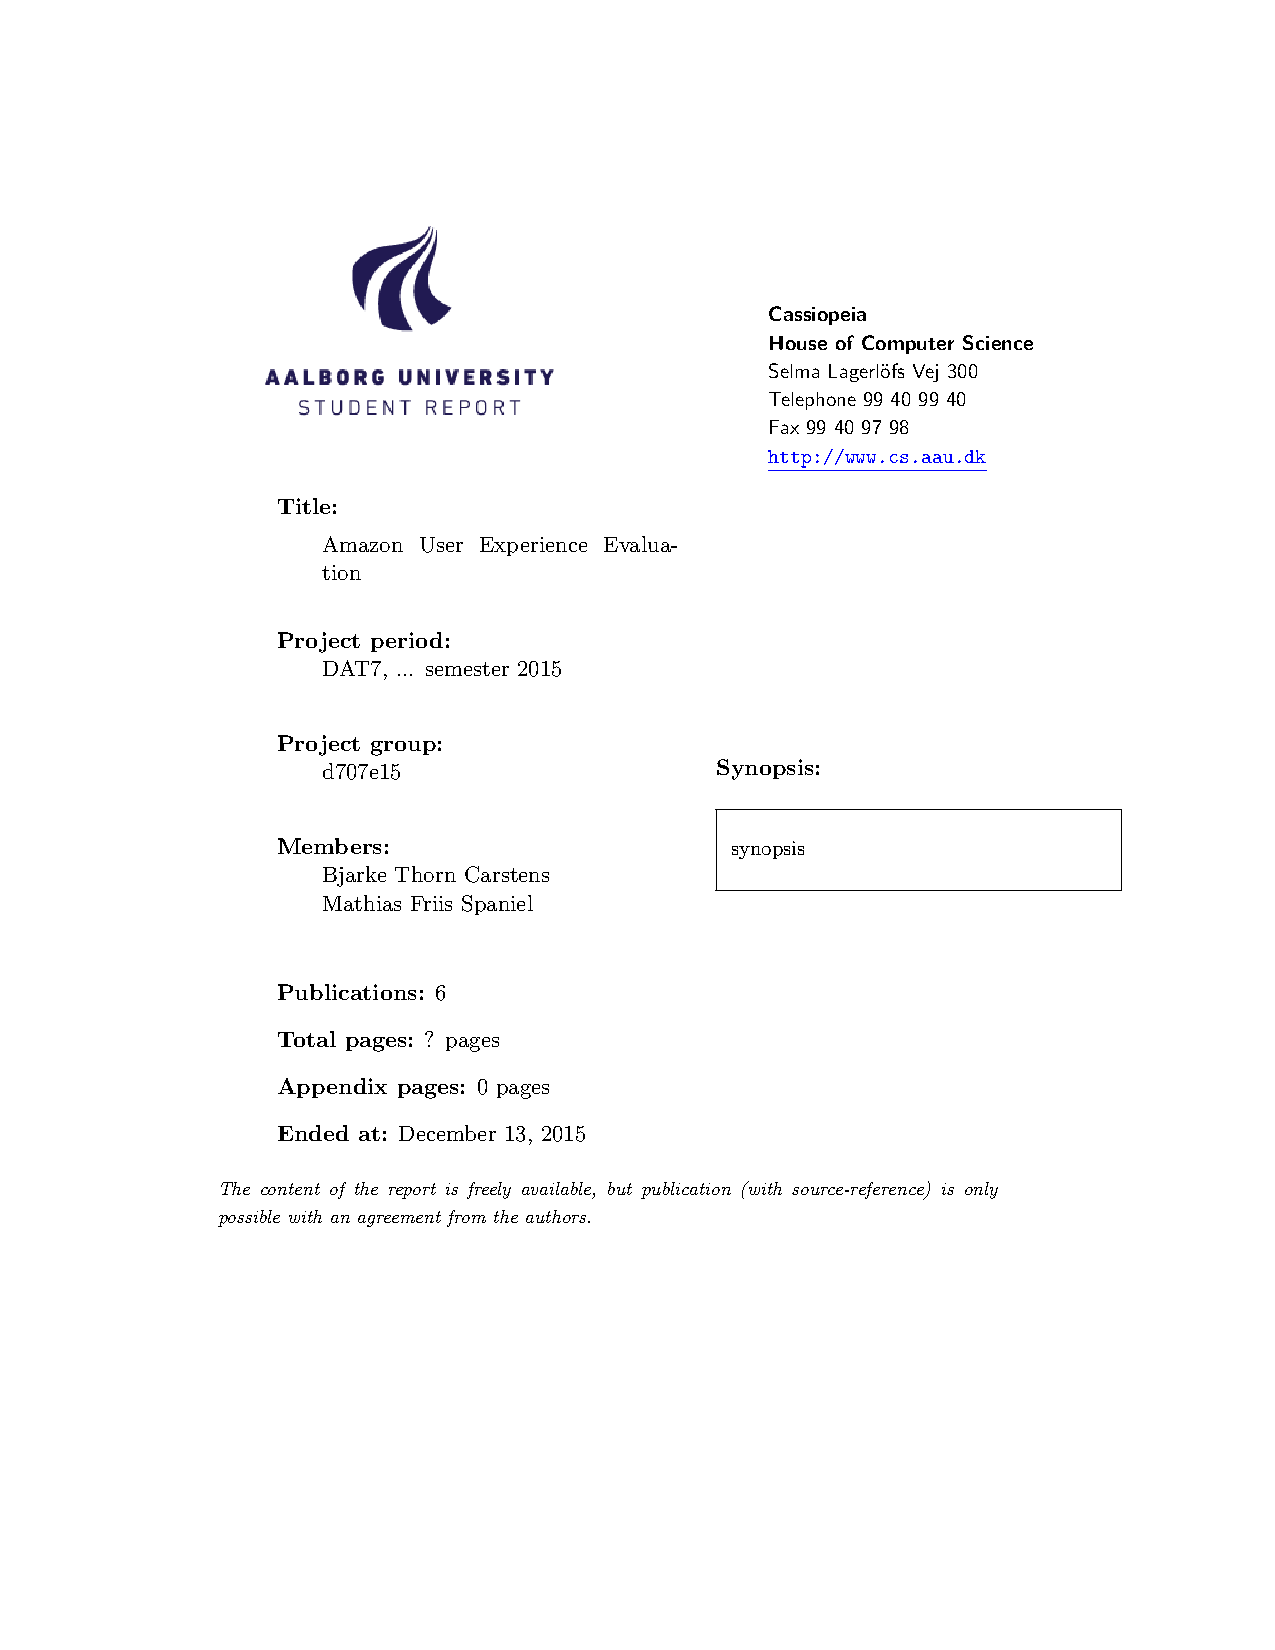
\includepdf[pages={1}]{titelblad.pdf}
%\newpage
%
%\begin{center}

\rule{\textwidth}{3pt}\\
\hrulefill\\
{ \huge \bfseries Preface} \\
\hrulefill\\
\rule{\textwidth}{3pt}\\
\end{center}

This article is a sixth semester bachelor thesis, written by a group of four students at Aalborg University at the Computer Science department. The article and experiments were performed in the period 2. February to 27. May.  

\begin{center}
\begin{minipage}{6cm}
\makebox[5cm]{}
\makebox[5cm]{}
\makebox[5cm]{\hrulefill}\\
Bjarke Thorn Carstens\\
\makebox[5cm]{}
\makebox[5cm]{}
\makebox[5cm]{\hrulefill}\\
Mathias Friis Spaniel \\
\end{minipage}
\end{center}
\vfill
{\large \today}

%\newpage

%\input{resume.tex}
%\newpage

\pagestyle{plain}
%\def\thepage{}
\setcounter{page}{1}

\begin{frontmatter}    

\title{Amazon user experience evaluation}

\author{\fnms{Bjarke Thorn} \snm{Carstens}}, \\ %
and
\author{\fnms{Mathias Friis} \snm{Spaniel}}

\address{Department of Computer Science, Aalborg University, Denmark}
%----------------------------------------------------------------------------------------


%\maketitle % Insert title

%\thispagestyle{fancy} % All pages have headers and footers

%----------------------------------------------------------------------------------------
%	ABSTRACT
%----------------------------------------------------------------------------------------

%\begin{abstract} 
%abstract, write abstract
%\end{abstract}
%
%\begin{keyword}
%Amazon, User Experience Evaluation, Attrakdiff, Co-discovery
%\end{keyword}
\end{frontmatter}

%----------------------------------------------------------------------------------------
%	ARTICLE CONTENTS
%----------------------------------------------------------------------------------------

%\begin{multicols}{2} % Two-column layout throughout the main article text

\section{Introduction} \label{sec:introduction}
...

%\lettrine[nindent=0em,lines=3]{L} orem ipsum dolor sit amet, consectetur adipiscing elit.
%\lipsum[2-3] % Dummy text

%------------------------------------------------

\section{Method description} \label{sec:experiments}
\subsection{Methods used for User Experience Evaluation}
AttrakDiff: Spørgeskema (7 pragmatisk og 14 hedonisk) \\
SUMI: Spørgeskema og test (test efterfulgt af spørgeskema til test af tilfredshed) \bjarke{originally chosen} \\
Co-discovery

%------------------------------------------------

\section{Evaluation process}
In order to structure the UX evaluation we created the following testplan, which is also meant to focus the evaluation and define milestones in the further development of the product.

\subsection{Testplan}
Our evaluation is formative, as our goal is to improve Amazon. \\ \\
\textbf{Purpose:} We want to test the user's experience and satisfaction of Amazon, both pragmatically and hedonically. \bjarke{explain why we want to do this (pragmatically and hedonically) and refer to hassenhahl 2003, explain}\\ \\
\textbf{Main questions:}
\begin{itemize}
\item Are there parts of the system the user is not satisfied with?
\item Which parts of the system did the user not use?
\item Are there parts of the system that is troublesome to the user?
\end{itemize}
\textbf{User profile:}
Ordinary Danes without a technical background. \\ \\
\textbf{Users and roles:}
One of us will function as a moderator and the other will be taking notes. Also our users are required to be capable of cooperating. \\ \\
\textbf{Test methods:}
\begin{itemize}
\item Questionares : AttrakDiff
\item Lab studies : Co-discovery
\end{itemize}
\textbf{Assignments:} The assignments are generally structured as stories with the intention of making the user explore the system, without guiding the user and keeping interaction with the user minimal. Examples of the stories used can be seen in \autoref{appendix:codiscovery} \\ \\
\textbf{Context and equipment:} In the context of the lab study we make use of the internet, a laptop for the users to use, a projector to be able to observe their interaction with the system during the evaluation, assignments to be solved by the users and a questionare in paper format. \\ \\
\textbf{Data collection:} Data is collected through the questionare and notes taken during the lab study.

\subsection{Description of evaluation process}
The evaluation of the system is done with a total of two participants, both male.

In order to evaluate the system we combine the two methods in the following manner: The two participants are present in the lab simultaneously, and are first read aloud an introduction detailing the purpose, and expectations, of the evaluation. The document specifying this can be found in \autoref{appendix:introductiontext}. They are then asked to sign a document specifying that they understand and accept the terms and conditions of the evaluation, see \autoref{appendix:codiscovery}.
The evaluation is now started using co-discovery, which the participants began by reading the current assignment aloud. While in the process of solving the assignments they were thinking aloud, and notified the moderator when they thought they had finished an assignment. The expected time of completion for co-discovery was 40 minutes, while the actual evaluation lasted only 17 minutes.

When the participants had solved all the assignments they were asked to fill in the AttrakDiff questionare, which took approximately 5 minutes.

Lastly a debriefing was performed to get an impression of the participants' experience using the system and of the evaluation process.
%\begin{itemize}
%\item Et par af to inde samtidig
%\item Oplæsning af introduktionstekst
%\begin{itemize}
%\item Hvordan opgaverne skal udføres
%\end{itemize}
%\item Blev først testet af co-discovery: moderator \& notetager
%\begin{itemize}
%\item Opgaver: Stories
%\item ~17 minutter i alt
%\end{itemize}
%\item Dern\ae st individuelt udfylde Attrakdiff spørgeskemaet
%\begin{itemize}
%\item ~5 minutter i alt
%\item Erfaring med amazon
%\end{itemize}
%\item Til sidst fælles evaluering
%\begin{itemize}
%\item Deltagers oplevelse af systemet
%\item Vores m\aa l med testen/opgaverne
%\end{itemize}
%\end{itemize}

%------------------------------------------------
\section{Results} \label{sec:results}
\subsection{Results for Co-discovery}
The functionality primarily used while trying to solve the assignments was the main search bar, located at the top center, see \autoref{results:amazonsearchbar}. As well as the sorting function of the found results for a given search, sorted primarily by price, see \autoref{results:amazonsortby}.

\begin{figure}[h]

\includegraphics[scale=0.3]{./includes/amazon_search_bar.png}
\label{results:amazonsearchbar}
\caption{Amazon main search bar}
\end{figure}

\begin{figure}[h]
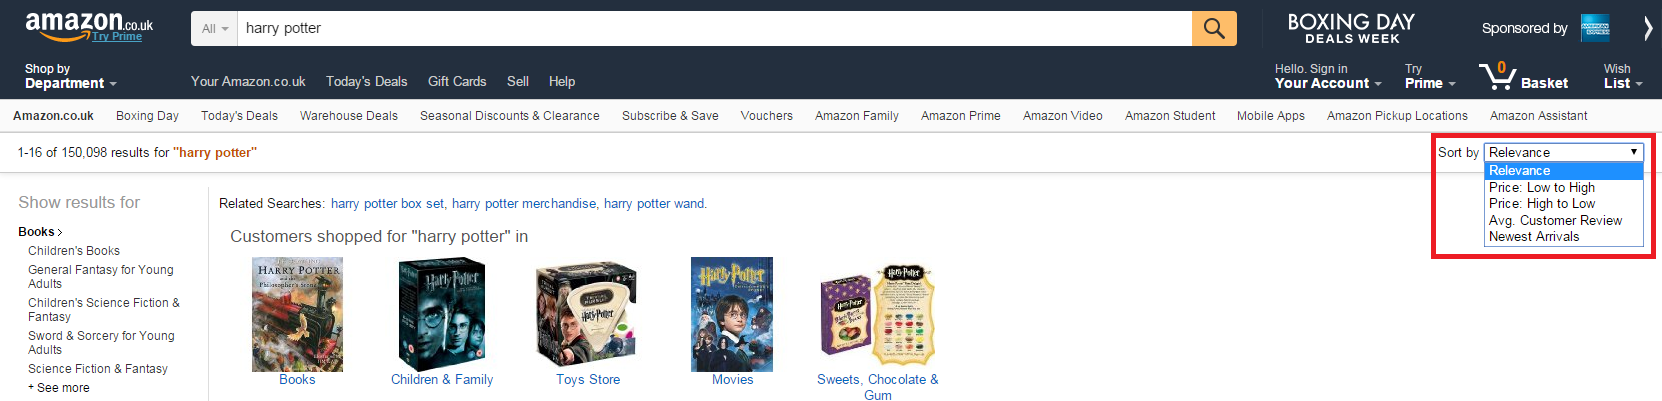
\includegraphics[scale=0.3]{./includes/amazon_sort_by.png}
\label{results:amazonsortby}
\caption{Amazon sort search result by}
\end{figure}
\bjarke{find tool to highlight important parts of pictures}

The functionality that we considered useful, and expected to be used, included the recommender system, and the category drop-down menu in the top left corner, which were never utilized, see \bjarke{insert pics}. Also the participants became rather confused when trying to find the relevant information regarding shipping of a certain product.

\subsection{Results for AttrakDiff}
The results of the AttrakDiff can be seen in ... below. \\

\bjarke{lav figur med resultater} \\

From the results of the AttrakDiff questionare we observed that the participants agreed that the system was
\begin{itemize}
\item Simple
\item Easy to use
\item Practical
\item Professional
\end{itemize}
However they didn't find it especially:
\begin{itemize}
\item Social
\item Innovative
\item Creative
\item New
\end{itemize}


%------------------------------------------------
\section{Discussion and conclusion} \label{sec:conclusion}
To answer the main questions specified in the testplan, we found that the amount of information contained on the product pages, caused the participants to be confused when searching for specific information, such as information regarding shipping. Another problem we noticed during the evaluation, was that product pages were structured in such a way that details about the given product was spread very widely across the page, which caused the participants to become frustrated.

As previously mentioned, we observed that they did not utilize the recommender system, among other functionality, even though we attempted to create assignments that facilitated exploration of Amazon. The primary reason for this, is that they found it more convenient to use the main search bar for navigation of the entire system. 

\subsection{For Co-discovery}
We found that using Co-discovery facilitated in more exploration of the system, as the participants naturally influenced each other during their use of the system. This in turn also made them less likely to interact with the moderator. Co-discovery also made it more natural to think aloud for the participants, in the sense that it took place in the form of an ongoing conversation. This interaction between the participants helped highlight their false assumptions regarding the system. 

However, the method has some cons as well. Due to the participants influencing each other, the method does not tell anything about how the individual would have interacted with the system. Another problem is that being able to perform the evaluation requires more resources, compared to methods requiring only one participant, partly because solving the logistics of scheduling participants, capable of cooperating, can be difficult and time consuming.

Some of the issues we encountered were related to the assignments we proposed. An example of such an issue is that the participants did not explore much of the product page. A cause for this may be that the assignments did not provide significantly motivation for it. A way to improve this, could be to make participants look up further product information forcing them to explore product pages in their entirety. 

We also experienced that some of our assignments were not formulated restrictively enough, causing the participants to explore less of the system.
Co-discovery works best for discovering pragmatic issues with a system, this is because the nature of solving assignments simply relate best to pragmatic features. If Co-discovery was to be used for testing the hedonic qualities of a system, this would have to be done in a similar way and hoping for a clear reaction from the participants related to hedonic features.

\subsection{For AttrakDiff}
We experienced that the AttrakDiff questionare was quick and simple to create, and that it was easy to get an overview of the opinions of all the participants. However, we found that the participants had a hard time interpreting the meaning of the questions. Another problem is the sample size, which was simply too small to make any conclusions. This suggests that AttrakDiff should be used in contexts that ensure a large number of participants, e.g. questionares by email. The questions are also not very informative, which makes it hard to make conclusions on why the participant thinks what he thinks, in turn making it hard to utilize the results. It can also occur that the participants don't put much effort into filling in the questions, rendering the results useless.

We think that the Danish translation helped, however it was clear that participants still have issues understanding the meaning of the questions, as mentioned earlier.

\subsection{Advice for Amazon}
To summarize, the overall problems identified in regards to UX on Amazon are:
\begin{itemize}
	\item Too much of information and hidden information.
	\item A lot of diversity and inconsistency in product pages in regards to information and functionality.
	\item A lot of functionality serving the same purpose, while quite a few of the features are not used. 
\end{itemize}

We propose the following advice for Amazon:

\begin{enumerate}
\item Make important hidden information more visible and accessible to the users.
\item Investigate whether it is possible to cut down on redundant information and functionality on product pages.
\item Restructure product pages to make them more consistent.
\end{enumerate}

\subsection{Preferred method}
Provided we were to perform another UX evaluation, under the same circumstances, we would choose to use the method Co-discovery. A reason for this is that it naturally facilitates interaction between the participants, which results in further exploration of the system. While AttrakDiff in this setting is rendered somewhat ineffective, due to the requirement of a large sample size.

\newpage

\section{Appendix}
\subsection{Attrakdiff questionare} \label{appendix:questionare}
\subsection*{Sp\o rgeskema}
Navn: \\
Alder: \\
Besk\ae ftigelse: \\



Jeg finder systemet...

\begin{table}[h]
\centering

\label{my-label}
\begin{tabular}{lll}
isolerende & $\bigcirc$ $\bigcirc$ $\bigcirc$ $\bigcirc$ $\bigcirc$ $\bigcirc$ $\bigcirc$ & socialt \\
ubehageligt & $\bigcirc$ $\bigcirc$ $\bigcirc$ $\bigcirc$ $\bigcirc$ $\bigcirc$ $\bigcirc$ & behageligt \\  
kompliseret & $\bigcirc$ $\bigcirc$ $\bigcirc$ $\bigcirc$ $\bigcirc$ $\bigcirc$ $\bigcirc$ & simpelt  \\
uprofessionelt & $\bigcirc$ $\bigcirc$ $\bigcirc$ $\bigcirc$ $\bigcirc$ $\bigcirc$ $\bigcirc$ & professionelt \\ 
grimt & $\bigcirc$ $\bigcirc$ $\bigcirc$ $\bigcirc$ $\bigcirc$ $\bigcirc$ $\bigcirc$ & attraktivt \\
upraktisk & $\bigcirc$ $\bigcirc$ $\bigcirc$ $\bigcirc$ $\bigcirc$ $\bigcirc$ $\bigcirc$ & praktisk   \\ 
besv\ae rligt & $\bigcirc$ $\bigcirc$ $\bigcirc$ $\bigcirc$ $\bigcirc$ $\bigcirc$ $\bigcirc$ & ligetil \\ 
uforudsigelig & $\bigcirc$ $\bigcirc$ $\bigcirc$ $\bigcirc$ $\bigcirc$ $\bigcirc$ $\bigcirc$ & forudsigeligt  \\
fremmedg\o rende & $\bigcirc$ $\bigcirc$ $\bigcirc$ $\bigcirc$ $\bigcirc$ $\bigcirc$ $\bigcirc$ & integrerende \\
upr\ae sentabelt & $\bigcirc$ $\bigcirc$ $\bigcirc$ $\bigcirc$ $\bigcirc$ $\bigcirc$ $\bigcirc$ & pr\ae sentabelt \\
afvisende & $\bigcirc$ $\bigcirc$ $\bigcirc$ $\bigcirc$ $\bigcirc$ $\bigcirc$ $\bigcirc$ & inviterende \\
fantasil\o st & $\bigcirc$ $\bigcirc$ $\bigcirc$ $\bigcirc$ $\bigcirc$ $\bigcirc$ $\bigcirc$ & kreativt \\
d\aa rligt & $\bigcirc$ $\bigcirc$ $\bigcirc$ $\bigcirc$ $\bigcirc$ $\bigcirc$ $\bigcirc$ & godt  \\
forvirrende & $\bigcirc$ $\bigcirc$ $\bigcirc$ $\bigcirc$ $\bigcirc$ $\bigcirc$ $\bigcirc$ & klart struktureret \\
frast\o dende & $\bigcirc$ $\bigcirc$ $\bigcirc$ $\bigcirc$ $\bigcirc$ $\bigcirc$ $\bigcirc$ & tiltr\ae kkende \\
konservativt & $\bigcirc$ $\bigcirc$ $\bigcirc$ $\bigcirc$ $\bigcirc$ $\bigcirc$ $\bigcirc$ & innovativt  \\
kedeligt & $\bigcirc$ $\bigcirc$ $\bigcirc$ $\bigcirc$ $\bigcirc$ $\bigcirc$ $\bigcirc$ & fangende \\
udfordrende & $\bigcirc$ $\bigcirc$ $\bigcirc$ $\bigcirc$ $\bigcirc$ $\bigcirc$ $\bigcirc$ & nemt  \\
afskr\ae kkende & $\bigcirc$ $\bigcirc$ $\bigcirc$ $\bigcirc$ $\bigcirc$ $\bigcirc$ $\bigcirc$ & motiverende  \\
normalt & $\bigcirc$ $\bigcirc$ $\bigcirc$ $\bigcirc$ $\bigcirc$ $\bigcirc$ $\bigcirc$ & nyt  \\
uh\aa ndterbart & $\bigcirc$ $\bigcirc$ $\bigcirc$ $\bigcirc$ $\bigcirc$ $\bigcirc$ $\bigcirc$ & h\aa ndterbart \\ 
kl\ae brigt ----remember this & $\bigcirc$ $\bigcirc$ $\bigcirc$ $\bigcirc$ $\bigcirc$ $\bigcirc$ $\bigcirc$ & stilfuldt  \\
skaber afstand til folk & $\bigcirc$ $\bigcirc$ $\bigcirc$ $\bigcirc$ $\bigcirc$ $\bigcirc$ $\bigcirc$ & bringer mig t\ae ttere p\aa \space folk
\end{tabular}
%\caption{My caption}
\end{table}

%\begin{Form}
%{Do you want to: }%
%\ChoiceMenu[radio,radiosymbol=\ding{109},name=myGroupOfRadiobuttons]{}{Do it all again=Again}
%\ChoiceMenu[radio,radiosymbol=\ding{52},name=myGroupOfRadiobuttons]{}{Pretend it never happened=Pretend}
%\ChoiceMenu[radio,radiosymbol=\ding{52},name=myGroupOfRadiobuttons]{}{Write a book about it=Write}
%\end{Form}

\subsection{Co-discovery} \label{appendix:codiscovery}
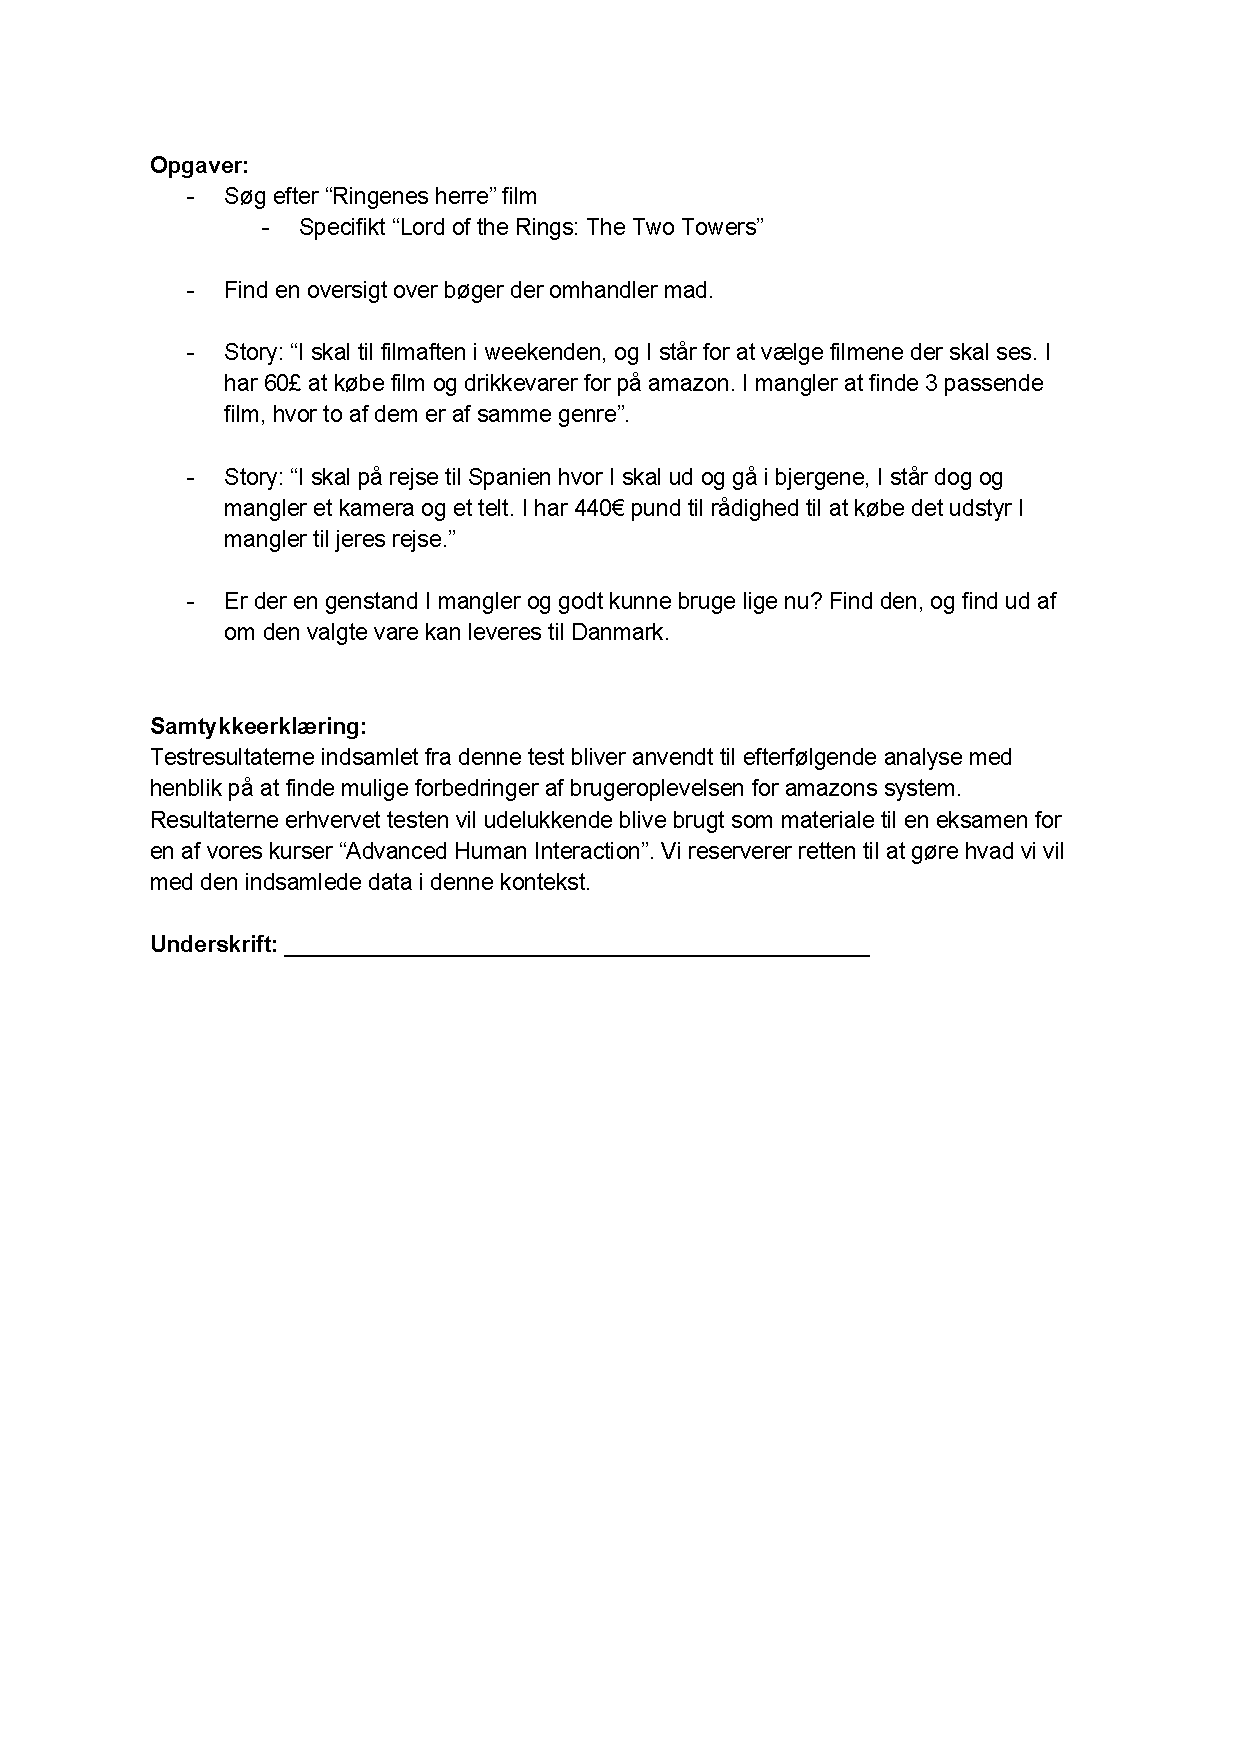
\includegraphics[scale=0.8]{./includes/opgaver_og_samtykkeerklaering.pdf}

\subsection{Introduction text} \label{appendix:introductiontext}
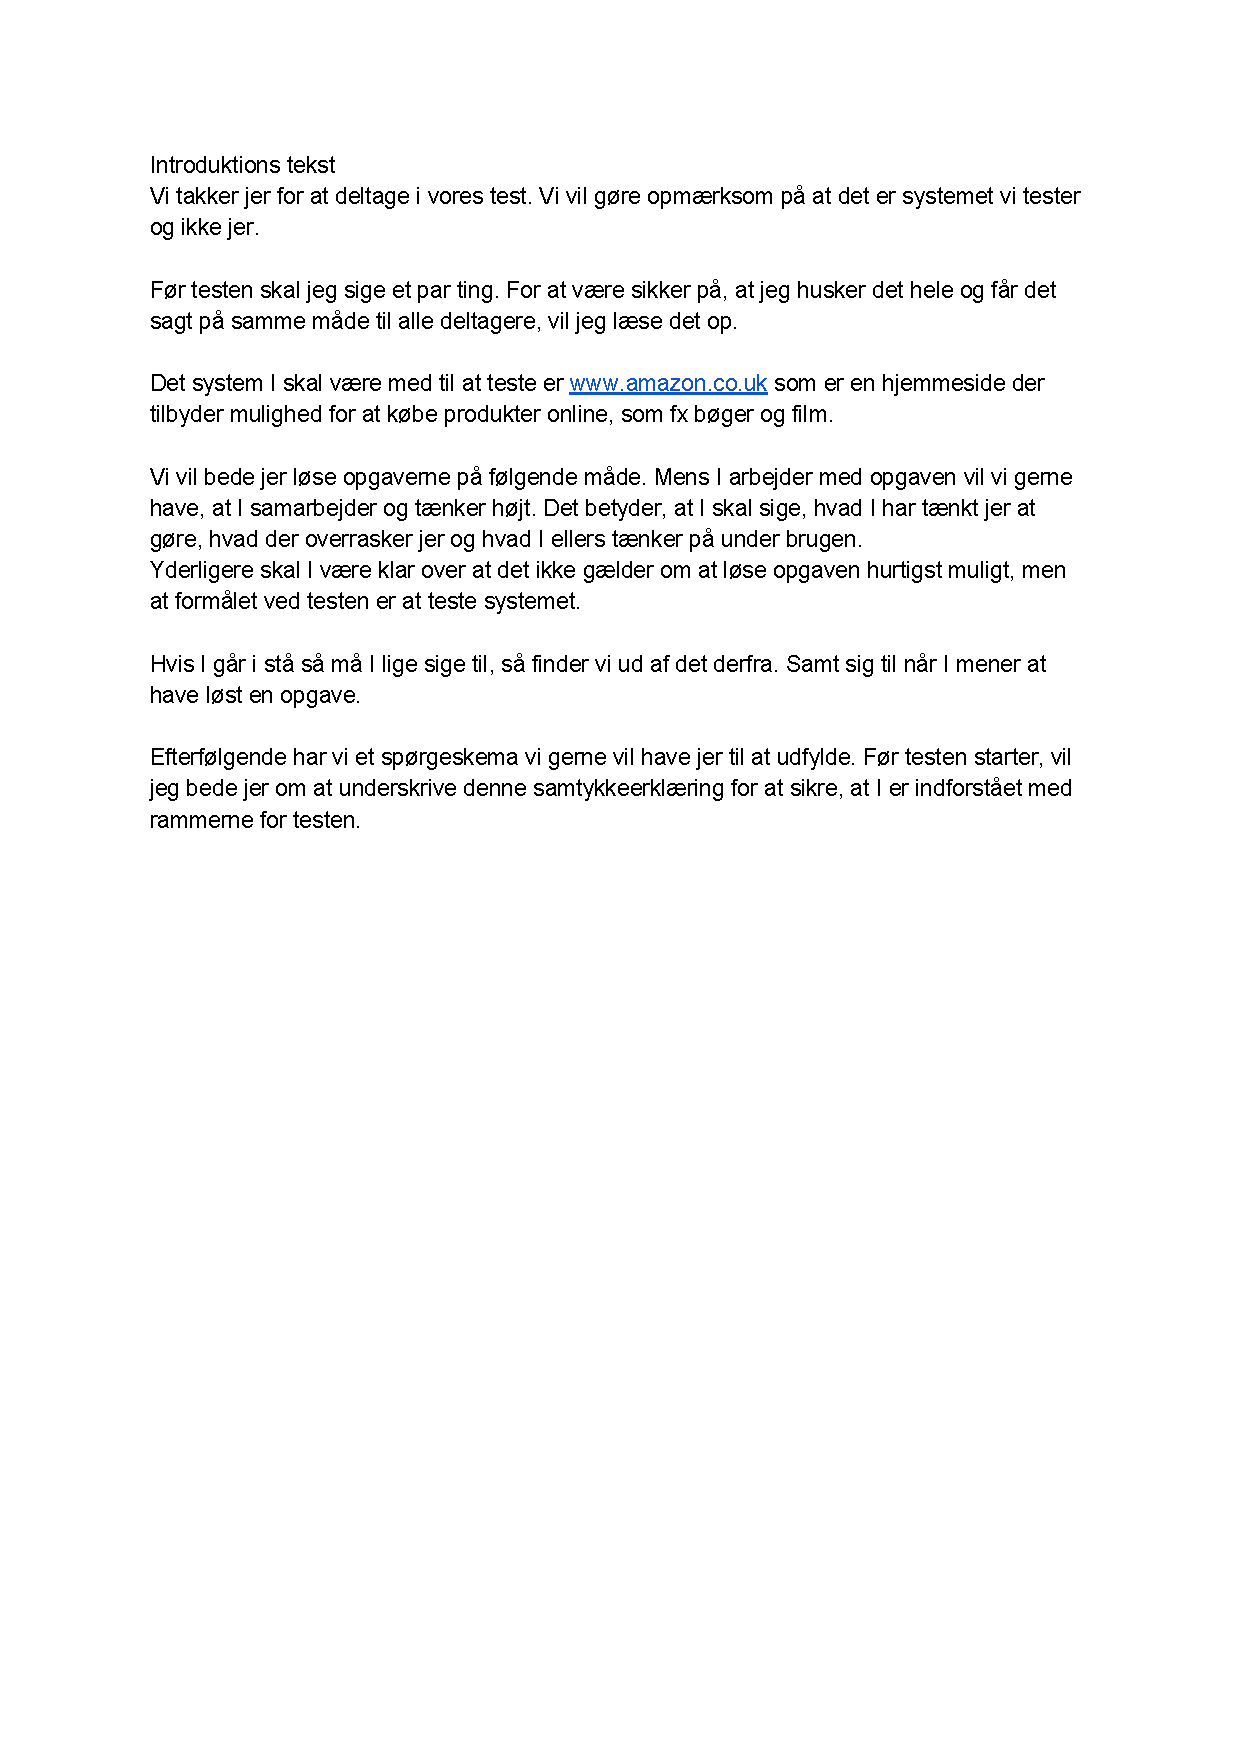
\includegraphics[scale=0.8]{./includes/introduktionstekst.pdf}

%\setboolean{@twoside}{false}
%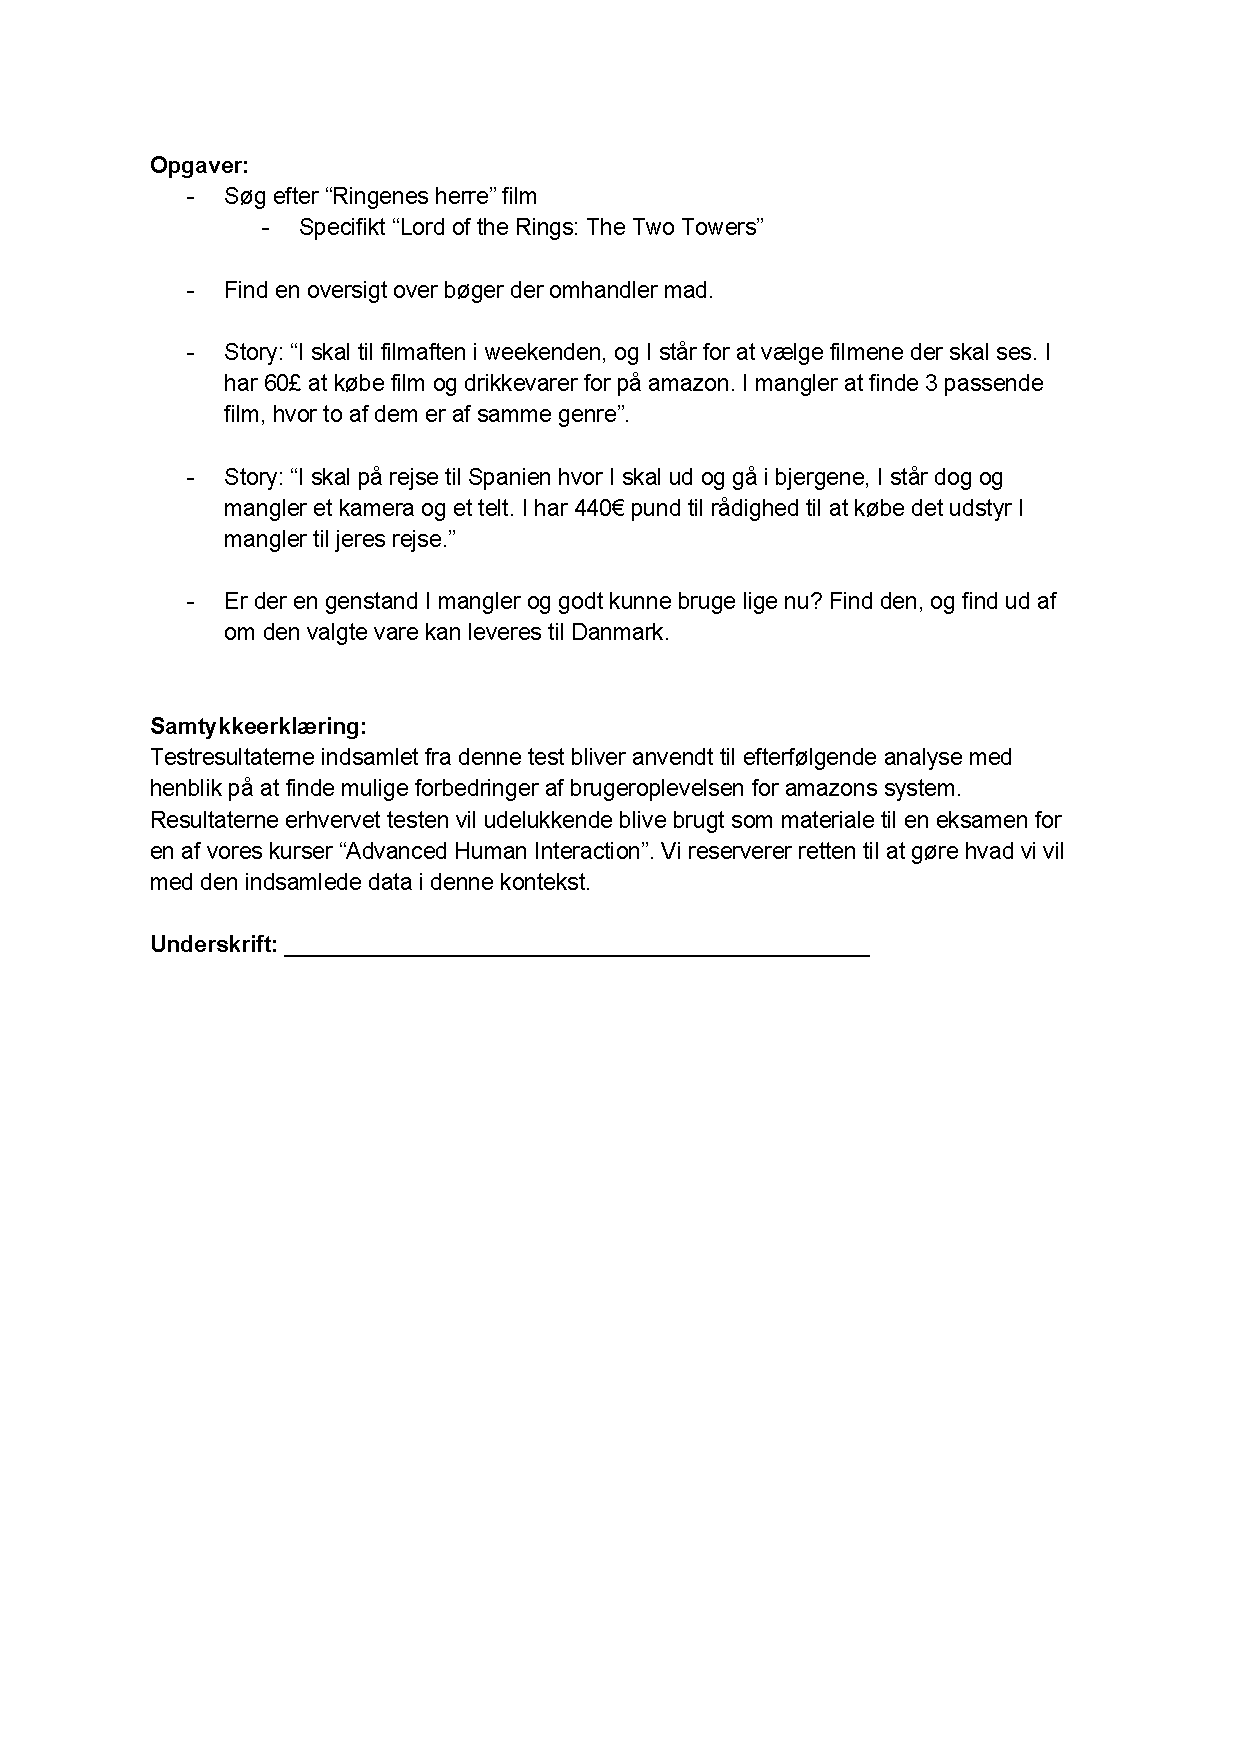
\includepdf[pages=-, offset=75 -75]{./includes/opgaver_og_samtykkeerklaering.pdf}
%%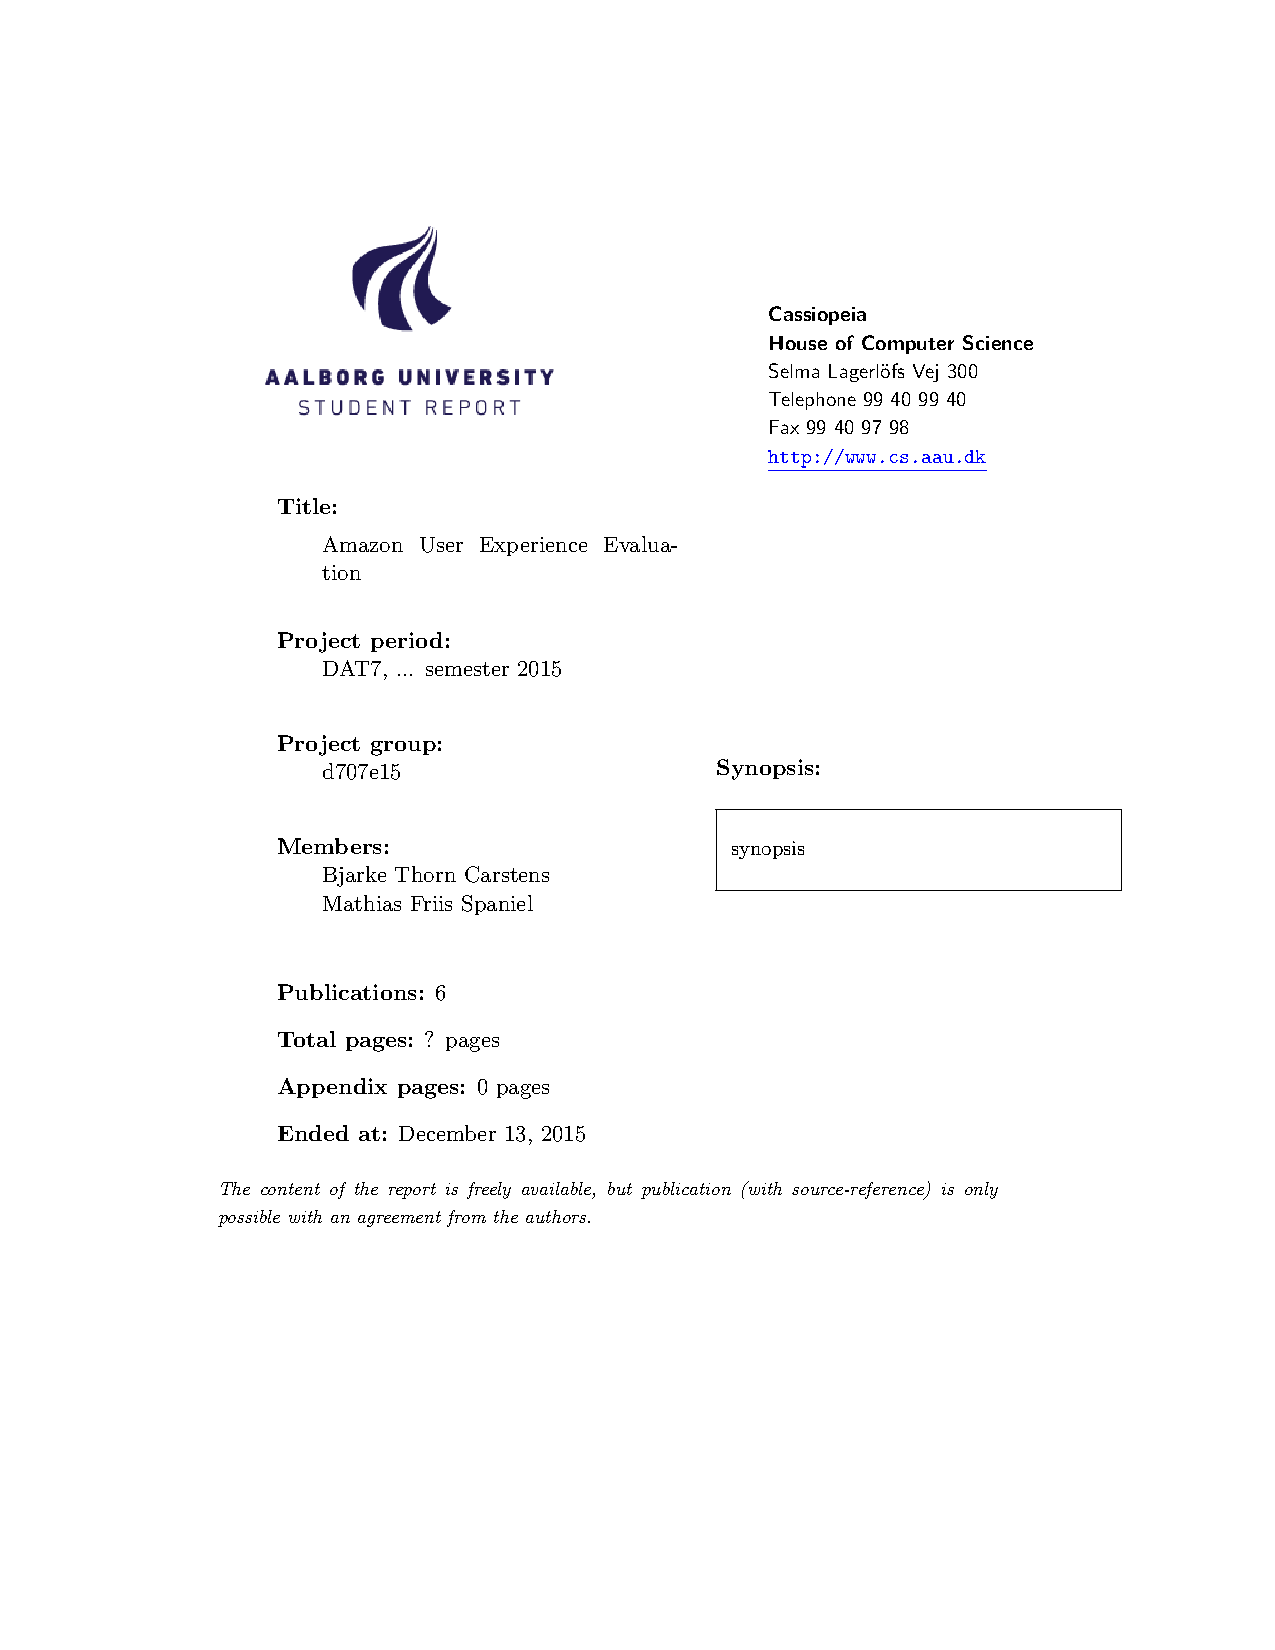
\includepdf[pages={1}]{titelblad.pdf}
%\newpage


%----------------------------------------------------------------------------------------
%	REFERENCE LIST
%----------------------------------------------------------------------------------------



\newpage

\bibliographystyle{unsrt}
\bibliography{biblo}
%\bibliographystyle{plainnat}



%\begin{thebibliography}{99} % Bibliography - this is intentionally simple in this template

%\bibitem[Figueredo and Wolf, 2009]{Figueredo:2009dg}
%Figueredo, A.~J. and Wolf, P. S.~A. (2009).
%\newblock Assortative pairing and life history strategy - a cross-cultural
 % study.
%\newblock {\em Human Nature}, 20:317--330.
 
%\end{thebibliography}

%----------------------------------------------------------------------------------------

%\end{multicols}

\end{document}